\documentclass[14pt, a4paper]{extarticle}

\usepackage[utf8]{inputenc}
\usepackage[russian]{babel}

\usepackage{geometry}
\geometry{
	right=0.39in,
	left=1.18in,
	top=0.3in,
	bottom=0.49in
}

\usepackage{indentfirst}
\setlength\parindent{1.25cm}

\usepackage{titlesec}
\titlespacing*{\section}{0pt}{10pt}{0pt}

\usepackage{titlesec}
\titleformat{\section}{\normalfont\bfseries}{}{0pt}{}
\titleformat{\subsection}{\normalfont\itshape}{}{0pt}{}	
	
\usepackage{setspace}
\onehalfspacing

\usepackage{hyperref}

\usepackage[pdftex]{graphicx}
\graphicspath{{png/}}
\DeclareGraphicsExtensions{.pdf,.jpeg,.png}

\usepackage{listings}
\usepackage{xcolor}
\lstset { %
	language=C++,
	backgroundcolor=\color{black!5}, % set backgroundcolor
	basicstyle=\footnotesize,% basic font setting
}

\def \deptName {МО ЭВМ}
\def \subjName {Системы реального времени на основе Linux}
\def \labNo {3}
\def \labName {Визуализация в RViz}

\def \groupNo {2303}
\def \studName {Канушин М.С.}
\def \proffName {Филатов А.Ю.}

\begin{document}
	
	\begin{titlepage}
	\begin{center}
		\textbf{МИНОБРНАУКИ РОССИИ \\
		САНКТ-ПЕТЕРБУРГСКИЙ ГОСУДАРСТВЕННЫЙ \\	
		ЭЛЕКТРОТЕХНИЧЕСКИЙ УНИВЕРСИТЕТ \\
		<<ЛЭТИ>> ИМ. В.И. УЛЬЯНОВА (ЛЕНИНА) \\
		Кафедра \deptName}
		
		\topskip0pt
		\vspace*{\fill}
			\bigskip\bigskip\bigskip\bigskip\bigskip
			\bigskip\bigskip\bigskip\bigskip\bigskip
			\textbf{ОТЧЕТ \\
			по лабораторной работе №\labNo \\
			по дисциплине <<\subjName>> \\
			Тема: \labName}
		\vspace*{\fill}
		
		\vspace*{\fill}
		\begin{tabular*}{\textwidth}{l @{\extracolsep{\fill}} r r}
			Студент гр. \groupNo & \noindent\rule{4cm}{0.4pt} & \studName \\
			Преподаватель        & \noindent\rule{4cm}{0.4pt} & \proffName \\
		\end{tabular*}
	
		\bigskip\bigskip\bigskip
		\bigskip\bigskip\bigskip
		
		Санкт-Петербург \\
		2018
	\end{center}
	\end{titlepage}
	\setcounter{page}{2}
	
	\section{Цель работы.}
	Устроить бои роботов. Один робот побеждает другого робота, когда его поражающий элемент совпадает по координатам с координатами другого робота. В качестве поражающего элемента предполагается использовать конец <<многоколенчатого нунчака>>, как на рис. \ref{fig:mesh1}.
	\begin{figure}[h]
		\centering
		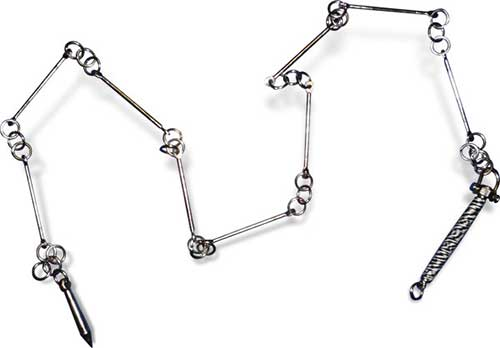
\includegraphics[width=2.5in]{b}
		\caption{Многоколенчатый нунчак}
		\label{fig:mesh1}
	\end{figure}
	Каждое сочленение вращается в плоской оси на 360 градусов.
	Точка В вращается вокруг точки С равномерно, образуя окружность, см. рис. \ref{fig:mesh2}.
	\begin{figure}[h]
		\centering
		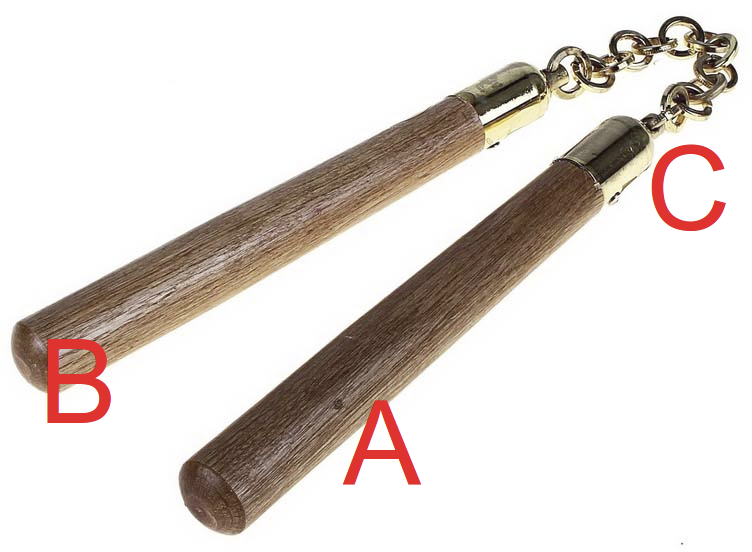
\includegraphics[width=2.5in]{a}
		\caption{Пример для одного сочленения ACВ}
		\label{fig:mesh2}
	\end{figure}
	Таких сочленений много, и итоговое положение конца нунчака относительно его начала становится почти непредсказуемым. Но именно этим концом и нужно попасть по сопернику.
	
	Плечи АС и ВС не обязательно должны быть равными. Скорость, с которой они вращаются задаётся вами.
	
	Интерфейс: можно использовать turtlesim и заставить черепашек бить других черепашек, но я рекомендую использовать rviz (там есть фигура "параллелепипед", который идеально сюда подойдёт).
	
	Интерактив: можно сделать обоих роботов управляемых ИИ, обоих ручными или одного такого, а другого такого.
	
	\section{Разработка программы.}
	\subsection{Роботы.}
	Каждый робот является объектом класса \textit{Robot}. Для него определены методы \textit{move\_<direction>} и \textit{stand\_still} для управления его местоположением, а так же метод \textit{hits} позволяющий определить попадание по роботу.
	
	Управление роботами происходит с помощью контроллера \textit{Controller}. В разработанной программе реализовано два вида контроллеров: ручной \\ \textit{ButtonController} и автоматический \textit{AiController}.
	
	Каждый робот обладает оружием со случайными параметрами.
	
	\subsection{Оружие.}
	Оружие состоит из узлов \textit{Node}, каждый из которых может вращаться вокруг своей оси. Для каждого оружия определены методы, позволяющие производить вращение и проверять попадания по роботам.
	
	\subsection{Визуализация.}
	Каждый робот представляется в RViz маркером-кубом, а узлы оружия - маркерами-стрелками. При изменении координат или повороте любого маркера, его отрисовка в RViz происходит заново. Такой механизм позволяет достаточно просто визуализировать смоделированное поведение роботов.
	
	\subsection{Алгоритм работы программы.}
	В функции \textit{main} создается 4 робота: 1 управляется с клавиатуры, остальные - в автоматическом режиме.
	
	В цикле начинают работать контроллеры, обеспечивающие передвижения роботов.
	
	Запускается два таймера. Один проверяет, что робот, управляемый человеком, не уничтожен, а второй - вращает оружия роботов в независимости от местоположения робота.
	
	При уничтожении робота, управляемого человеком, алгоритм прекращает свою работу и программа завершается.

	\section{Код программы.}
	Код программы представлен в репозитории по адресу \url{https://github.com/Rextuz/ros_2017/tree/master/2303/Kanushin/lab3}
	
\end{document}